\documentclass{article}\usepackage{graphicx} % new way of doing eps files
\usepackage{listings} % nice code layout
\usepackage[usenames]{color} % color
\usepackage{float}
\definecolor{listinggray}{gray}{0.9}
\definecolor{graphgray}{gray}{0.7}
\definecolor{ans}{rgb}{1,0,0}
\definecolor{blue}{rgb}{0,0,1}
% \Verilog{title}{label}{file}
\newcommand{\Verilog}[3]{
  \lstset{language=Verilog}
  \lstset{backgroundcolor=\color{listinggray},rulecolor=\color{blue}}
  \lstset{linewidth=\textwidth}
  \lstset{commentstyle=\textit, stringstyle=\upshape,showspaces=false}
  \lstset{frame=tb}
  \lstinputlisting[caption={#1},label={#2}]{#3}
}


\author{Christopher Leger}
\title{Lab1: Barrel Shifters}

\begin{document}
\maketitle

\section{Introduction}
The purpose of this was to test the various designs of barrel shifters which include the case design, where each possible shift is made, or the stage design, where shifts are made in powers of two to total the number of possible shifts. These shifters were design for both eight and sixteen bits to show the extension of these designs. There are also two different designs for choosing whether the shift is to the left or the right that are being shown throughout the lab. 
\section{Interface}
All of the shifters take in the amount of bits specified by the shifter, either eight or sixteen bits. Then the shifters require a value to describe how many shifts the user wants. For the eight bit shifters this value is three bits long and for the sixteen bit shifters this value is four bits long. The shifters then output the shifted bits with the same number of bits as the input. The next level up, the designs for choosing left or right shift both take in the same values as their associated shifters but also take in and extra one bit input that is the bit that decides which shift to use. The top module that is implemented on the board uses the switches to set the values passed to the shifters and the buttons for both the choice of left or right and the amount of shifts that are to be performed. 
\section{Design}
There were two kinds of shifters designs, one where there were multiple stages of muxs to decide how many times to shift and one where a large mux was used to decide and the bits were shifted exactly the number they needed to in on movement. These designs were then expanded to fit sixteen bit inputs to evaluate how easily these designs can be made to work for larger inputs. The eight bit stage design is show in Figure~\ref{fig:StageShifter} and the eight bit case design is shown in Figure ~\ref{fig:CaseShifter}. Then to show the how these designs escalate to higher amounts of inputs, the sixteen bit designs are shown in Figures~\ref{fig:StageShifter16} and~\ref{fig:CaseShifter16}. The sixteen bit stage design requires less wiring and only added one more mux whereas the case design requires several wires to be added to the original mux but requires no extra muxs.
\begin{figure}[H]
\begin{center}
	\caption{Design for stage shifter.}\label{fig:StageShifter}
	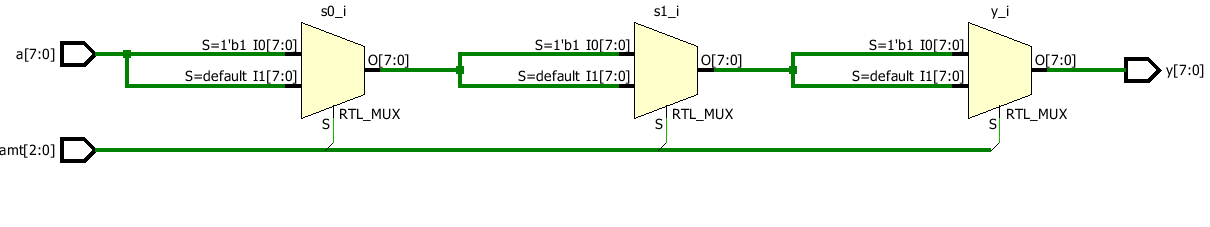
\includegraphics[width=1.2\textwidth]{../images/Shifter_stage_design.png}
\end{center}
\end{figure}
\begin{figure}[H]
\begin{center}
	\caption{Design for case shifter.}\label{fig:CaseShifter}
	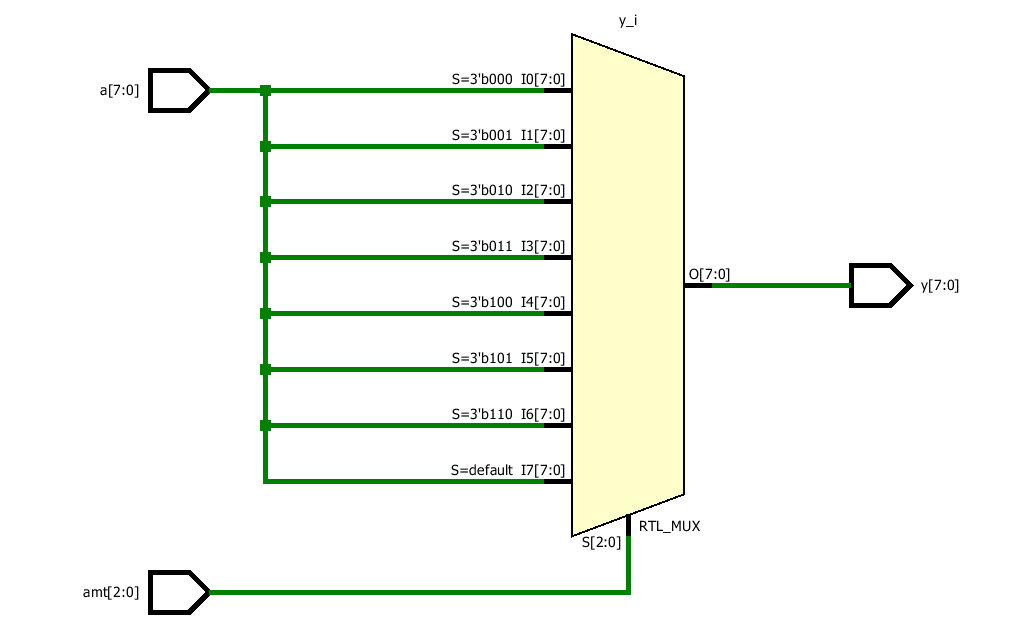
\includegraphics[width=0.7\textwidth]{../images/Shifter_case_design.png}
\end{center}
\end{figure}
\begin{figure}[H]
\begin{center}
	\caption{Design for stage shifter with 16bits.}\label{fig:StageShifter16}
	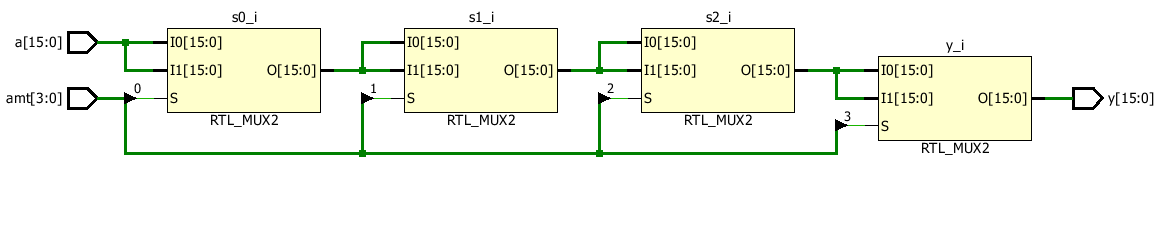
\includegraphics[width=1.2\textwidth]{../images/Shifter_stage_16bit_design.png}
\end{center}
\end{figure}
\begin{figure}[H]
\begin{center}
	\caption{Design for case shifter with 16bits.}\label{fig:CaseShifter16}
	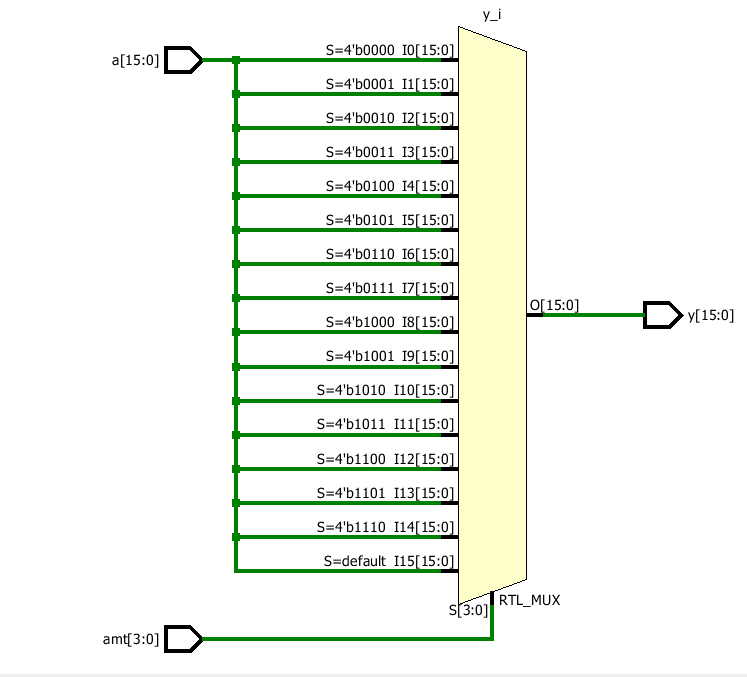
\includegraphics[width=0.7\textwidth]{../images/Shifter_case_16bit_design.png}
\end{center}
\end{figure}
The level above the individual shifters, where the decision between left or right shift is made, also has two possible designs. These include a design where the input is given to both a left and a right shifter and then a mux is used to decide which result to use, shown in Figure~\ref{fig:Left/Right}, and a design where an extra two wires are used, one to reverse the bits before the shifter which is fed to a mux with the original input and then one after the shifter to reverse the bits back to their original order but shifter to the right seen in Figure~\ref{fig:reverse/left}. The shifter used in the second design is only a left shifter but reversing the bits and then reversing them back is effectively a shift right. The figures show these designs using sixteen bits and the stage shifters but both types of shifter, stage and case, and both eight and sixteen bits were used during later implementation. 
\begin{figure}[H]
\begin{center}
	\caption{Design for shift left and right choice.}\label{fig:Left/Right}
	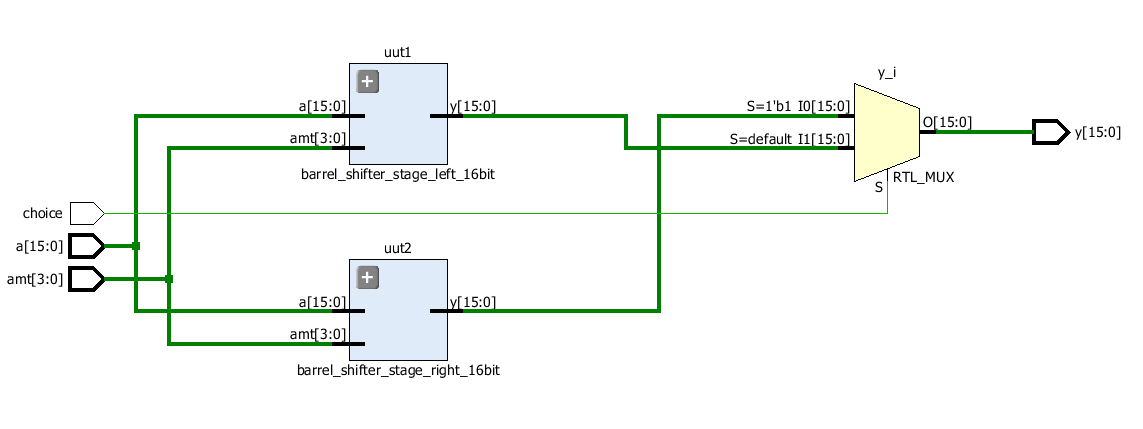
\includegraphics[width=1.0\textwidth]{../images/Shifters.png}
\end{center}
\end{figure}
\begin{figure}[H]
\begin{center}
	\caption{Design for shift left with possible reverse bits.}\label{fig:reverse/left}
	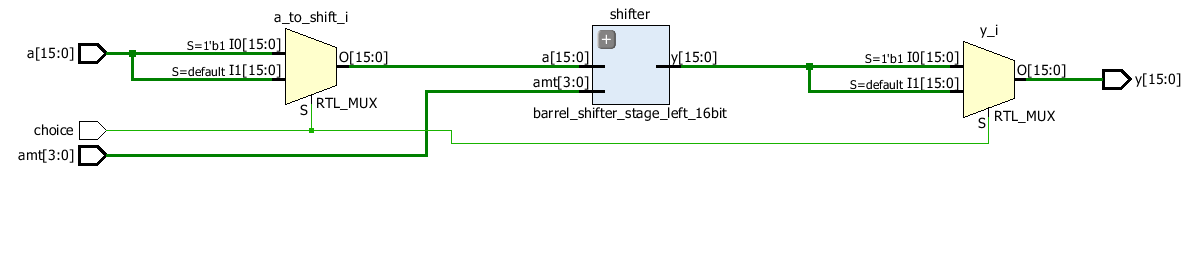
\includegraphics[width=1.0\textwidth]{../images/Shift_left_or_right.png}
\end{center}
\end{figure}
\section{Implementation}
Various methods were used to implement each of the designs for both the shifters and the higher level modules. The stage designs of the shifters use dataflow implementation where assign statements and the query operator are used to create two input one output muxs that are then cascaded to create the larger shifts. The sixteen bit implementation requires one more assign statement than the eight bit version because it needs a mux that can shift the bits eight positions so that up to fifteen shifts can be made which, as the number of bits increases can cause a delay in output due to how far a value has to travel to move through all of the possible muxs. The code to implement these with both left and right shifts can be seen in Listings~\ref{code:StageShift} and~\ref{code:StageShift16} for the eight and sixteen bits, respectively. The case designs use behavioral implementation in order to create on mux that has all of the possible inputs and only one output which can only be guaranteed by behavioral design. The sixteen bit implementation has eight more inputs to the mux than the eight bit design and these implementations can be seen in Listings~\ref{code:CaseShift} and~\ref{code:CaseShift16}. As the number of bits increases the mux will need more inputs which may later cause a fanin problem. Both of the case designs use an "always@*" block, which means that these implementations are for combinational circuits as they do not use a clock to tell them when to move to the next instruction. This is true for the stage designs as well but those are shown by being dataflow style codes. \par 


\Verilog{Verilog code for Stage Shifter.}{code:StageShift}{../code/common/list_ch03_19_barrel_shifter_stage.v}
\Verilog{Verilog code for Stage Shifter with 16bits.}{code:StageShift16}{../code/common/barrel_shifter_stage_16bit.v}
\Verilog{Verilog code for Case Shifter.}{code:CaseShift}{../code/common/list_ch03_18_barrel_shifter_case.v}
\Verilog{Verilog code for Case Shifter with 16bits.}{code:CaseShift16}{../code/common/barrel_shifter_case_16bit.v}

The higher level codes for choosing between left or right shifts both use dataflow coding, shown by the use of "assign" to create the muxs used for choosing between left or right shift because it is the easiest method for creating a two to one mux. The rest of the modules just use wires and calls to the shifters to create the correct effect on the inputs. The code shown in Listings~\ref{code:Shifters} and~\ref{code:reverseLeft} only shows one implementation of these modules but for testing and simulation these were made with each stage and case shifters as well as for both eight and sixteen bits. There are eight implementations total of these top modules despite the fact that only two are shown. The other implementations are very similar with the only difference between case and shift being which of the shifters was called in the higher module and the difference between eight and sixteen being that the size of each input and output increased.

\Verilog{Verilog code for shift left and right choice.} {code:Shifters}{../code/common/Shifters_stage_16bit.v}
\Verilog{Verilog code for shift left with possible reverse bits.}{code:reverseLeft}{../code/common/Shift_left_or_right_case_16bit.v}

\section{Test Bench Design}
The test benches designed test several different values of input and every possible shift for the individual shifters both eight and sixteen bit. Random values were passed to the shifters including the simple value of 1 to see where one bit was shifted to after each motion. Only one of the eight bit test benches is shown in Listing~\ref{code:ShifterTest} but these values are similar for the sixteen bit tests and for the eight bit case test. The upper level modules were all tested using the same test vectors where values similar to those used in the individual shifters but now the choice changes between the different values as well as during one of the constant values. Similar to how only one was shown for the individual shifters, only one test bench will be shown for the higher level but all eight cases were given the same tests as in Listing~\ref{code:HigherTest}.

\Verilog{Verilog code for testing the stage shifter.} {code:ShifterTest}{../code/common/Shifter_stage_test.v}
\Verilog{Verilog code for testing the higher level shifter choice.} {code:HigherTest}{../code/common/Shifters_16bit_test.v}

\section{Simulation}
The simulations created from the shown test benches showed that each of the possible shifters functions as expected and other than the occasional syntax error that was corrected quickly there were no large errors in the simulation of these test benches. The simulations can be seen in Figure~\ref{fig:ShifterTestSim} for the individual shifters and Figure~\ref{fig:HigherTestSim} for the higher level shifter choice modules. The simulations only show part of the test but do show the value changing and the shift amount changing as well as the direction of the shift altering. 
\begin{figure}[H]
\begin{center}
	\caption{Simulation for individual shifters test.}\label{fig:ShifterTestSim}
	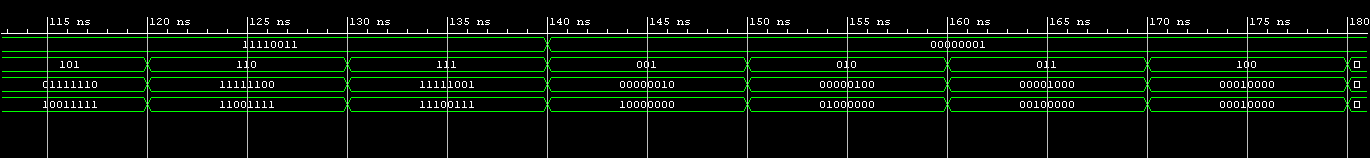
\includegraphics[width=1.5\textwidth]{../images/ShifterStageSim.png}
\end{center}
\end{figure}
\begin{figure}[H]
\begin{center}
	\caption{Simulation for higher level shifter choice test.}\label{fig:HigherTestSim}
	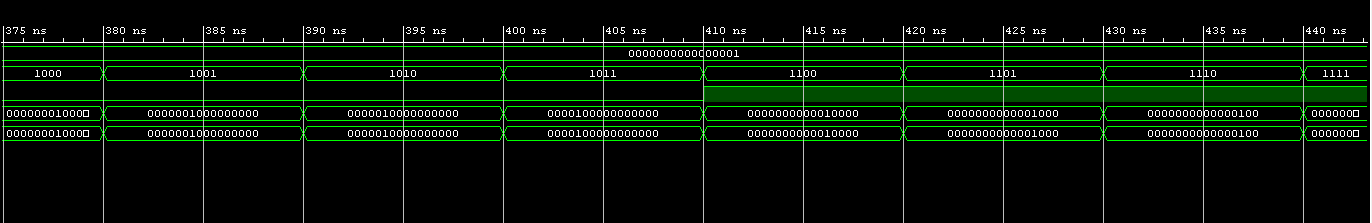
\includegraphics[width=1.5\textwidth]{../images/Shifters_16bit_sim.png}
\end{center}
\end{figure}
\section{FPGA Realization and Final Verification}
Only two versions of the higher level modules were fully realized on the FPGA. These were the left and right stage shifter with eight bits and the left and reverse left case shifter with sixteen bits. The switches were used to provide the bits to shifter and the buttons were used to decide which direction(press upper button for right shift) and how far to shift the bits. The full realization can be seen in Listing~\ref{code:8bitboard} for the eight bit version and Listing~\ref{16bitboard} for the sixteen bit versions. Both functioned properly when realized and verified on the board showing no discernible difference between the two designs when only shifting a few bits.

\Verilog{Verilog code for eight bit FPGA realization.} {code:8bitboard}{../code/common/pass_through_shifter.v}
\Verilog{Verilog code for sixteen bit FPGA realization.} {code:16bitboard}{../code/common/pass_through_shifter_16bit.v}

\section{Conclusions}
The final design chosen makes no discernible difference when only shifting the bits on an FPGA but can have a larger effect if that output is need for many things or if several different shifts on different values are made. The stage based design is significantly easy for the programmer to write and scale up but has a latency issue when expanded to more bits and the case based design has the benefit of being faster but is more difficult on the programmer and has a potential fanin issue when the number of bits increases. As for the higher level design, the left and right shift option is easier to visualize and implement and but if several bits need to be shifted it will take longer to shift both left and right and then decide which to use and the left and reverse left option is faster because it only shifts once but is more difficult to understand and remember that the bits need to be reversed back. There is now a much greater understanding of the difference that a design choice can make.
\end{document} 